% Author: Izaak Neutelings (Februari, 2020)
% http://texample.net/tikz/examples/tag/circuitikz/
% http://texample.net/tikz/examples/circuitikz/
% https://www.overleaf.com/learn/latex/CircuiTikz_package
% http://texdoc.net/texmf-dist/doc/latex/circuitikz/circuitikzmanual.pdf
% http://repositorios.cpai.unb.br/ctan/graphics/pgf/contrib/circuitikz/circuitikzmanual.pdf
\documentclass[border=5pt,tikz]{standalone}
\usepackage{amsmath} % for \dfrac
\usepackage{physics}
\usepackage{tikz,pgfplots}
\usepackage[siunitx]{circuitikz} %[symbols]
\usepackage[outline]{contour} % glow around text
\usetikzlibrary{arrows,arrows.meta}
\usetikzlibrary{decorations.markings}
\usetikzlibrary{hobby}
\tikzset{>=latex} % for LaTeX arrow head
\usepackage{xcolor}
\colorlet{Icol}{blue!50!black}
\colorlet{Ccol}{orange!90!black}
\colorlet{Rcol}{green!50!black}
\colorlet{loopcol}{red!90!black!25}
\colorlet{pluscol}{red!60!black}
\colorlet{minuscol}{blue!60!black}
\newcommand\EMF{\mathcal{E}} %\varepsilon}
\contourlength{1.5pt}

\ctikzset{capacitors/width=0.4}
\tikzstyle{EMF}=[battery1,l=$\EMF$,invert]
\tikzstyle{internal R}=[R,color=Rcol,Rcol,l=$r$,/tikz/circuitikz/bipoles/length=30pt]
\tikzstyle{loop}=[->,red!90!black!25]
\tikzstyle{loop label}=[loopcol,fill=white,scale=0.8,inner sep=1]
\tikzstyle{thick R}=[R,color=Rcol,thick,Rcol,l=$R$]
\tikzstyle{thick C}=[C,thick,color=Ccol,Ccol]
\tikzstyle{myswitch}=[closing switch,line width=0.3] %-{Latex[length=3]},

\begin{document}

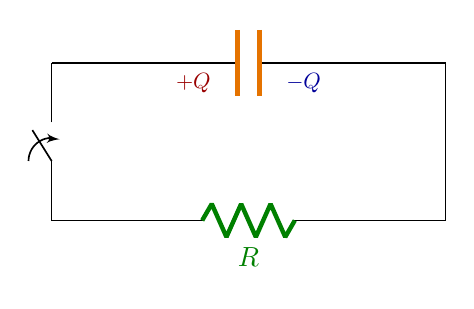
\begin{tikzpicture}
  \def\ang{220}
  \def\a{0.9}
  \def\b{0.8}

  \draw (0,0) to[thick C] (5,0) -- (5, -2)
              to[thick R] ++(-5,0) to[myswitch] (0,0);
  \node[minuscol,scale=0.8] at (3.2,-0.25) {$-Q$};
  \node[pluscol,scale=0.8] at (1.8,-0.25) {$+Q$};

\end{tikzpicture}

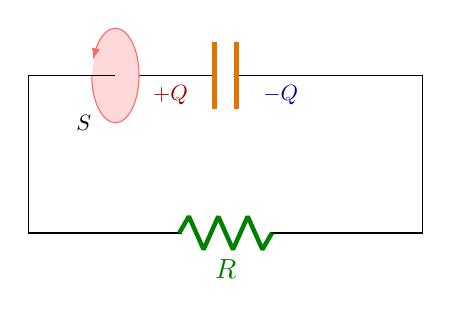
\begin{tikzpicture}
  \def\ang{220}
  \def\a{0.9}
  \def\b{0.8}

%   \filldraw [-latex, color=red!60, fill=red!15 ] (1,0) arc [start angle=-180, end angle=160, x radius=0.3, y radius=0.6];
%   \draw (0,0) -- (1.1, 0);
  \draw (0, 0) to[thick C] (5,0) -- (5, -2)
              to[thick R] ++(-5,0) -- (0,0);
  \node[minuscol,scale=0.8] at (3.2,-0.25) {$-Q$};
  \node[pluscol,scale=0.8] at (1.8,-0.25) {$+Q$};

    \filldraw [-latex, color=red!60, fill=red!15 ] (0.8,0) arc [start angle=-180, end angle=160, x radius=0.3, y radius=0.6];
  \node[scale=0.8] at (0.7, -0.6) {$S$};
  \draw (0,0) -- (1.1, 0);

	
\end{tikzpicture}

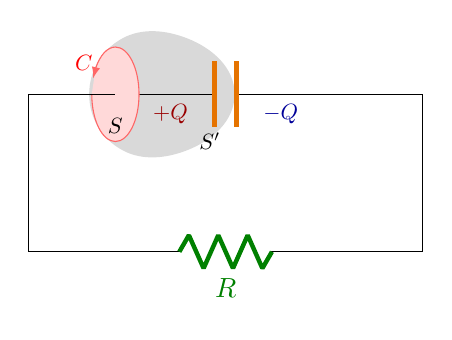
\begin{tikzpicture}
    \def\ang{220}
     \def\a{0.9}
    \def\b{0.8}

    \draw[thick, color=gray!30, fill=gray!30] (1.2,0.7) to[closed, curve through ={  (2.0,0.7) (2.6, 0) (2.0,-0.7) }] (1.2, -0.7);
    \draw (0, 0) to[thick C] (5,0) -- (5, -2)
              to[thick R] ++(-5,0) -- (0,0);
    \node[minuscol,scale=0.8] at (3.2,-0.25) {$-Q$};
    \node[pluscol,scale=0.8] at (1.8,-0.25) {$+Q$};
    

    \filldraw [-latex, color=red!60, fill=red!15 ] (0.8,0) arc [start angle=-180, end angle=160, x radius=0.3, y radius=0.6];
    \node[scale=0.8] at (1.1, -0.4) {$S$};
    \node[scale=0.8, red] at (0.7, 0.4) {$C$};
    \node[scale=0.8] at (2.3, -0.6) {$S'$};
  \draw (0,0) -- (1.1, 0);

	
\end{tikzpicture}
\end{document}